\documentclass[11pt,a4paper,twoside,french,svgnames]{report}
\usepackage[utf8]{inputenc} % force the use of utf8
\usepackage{lmodern}
\usepackage[T1]{fontenc} % font encoding, allows accents
\usepackage[papersize={21cm,29.7cm},top= 2.5cm,bottom=2.5cm, inner=2.5cm, outer=2.5cm]{geometry} % page formatting
\usepackage[francais]{babel} % translate everything in the desired language: table of contents, etc. 'english' can be replaced with 'francais'
\usepackage{graphicx} % images management
\usepackage{wrapfig} % floating images
\usepackage{array} % allow arrays
\usepackage{fancyhdr} % headers/footers management (overrides empty, plain and headings)
\usepackage{listings} % code insertion (MUST BE WRITTEN AFTER BABEL)
%\usepackage[nottoc,numbib]{tocbibind} % bib in toc
%\usepackage{pdfpages} % include PDF documents
\usepackage{enumitem} % for /setlist
\usepackage{color,soul} % add some colors and hightlight
\usepackage{xcolor} % more colors
\usepackage{textcomp}
\usepackage[hyphens]{url} % auto break lines in URL
\usepackage[hidelinks,  colorlinks  = true, % no borders, colors enabled
                        anchorcolor = blue,
                        linkcolor   = black, % links in table of contents
                        urlcolor    = blue,
                        citecolor   = blue]{hyperref}
%\usepackage[%nonumberlist,% no page number
%            toc,% displayed in toc
%            numberedsection,% displayed as a numbered section in toc
%            xindy]{glossaries} % glossary with xindy style. MUST BE WRITTEN AFTER HYPERREF
%\setglossarystyle{listgroup}

\sethlcolor{cyan} % package soul
\newcommand{\file}[1]{\hl{\emph{#1}}} % highlight a file URI

%\makeglossaries
%\loadglsentries{glossary.tex}

%%%%%%%%%%%%%%%%%%%%%%%%%%%%%%%%%%%%%%%%%%%%%%%%%%%%%%%% LISTINGS %%%%%%%%%%%%%%%%%%%%%%%%%%%%%%%%%%%%%%%%%%%%%%%%%%%%%%%%
\definecolor{comment}{rgb}{0.12, 0.38, 0.18 } % adjusted, in Eclipse: {0.25, 0.42, 0.30 } = #3F6A4D
\definecolor{keyword}{rgb}{0.37, 0.08, 0.25}  % #5F1441
\definecolor{string}{rgb}{0.06, 0.10, 0.98} % #101AF9

\lstset{
  columns=flexible, %prevent extra spaces
  rulecolor=\color{black!50},
  backgroundcolor = \color{blue!10},
  numbers=none, % line numbering
  showspaces=false,
  showtabs=false,
  tabsize=4,
  breaklines=true,
  showstringspaces=false,
  breakatwhitespace=false,
  commentstyle=\color{comment},
  keywordstyle=\color{keyword},
  stringstyle=\color{string},
  basicstyle=\ttfamily,
  extendedchars=true,
  emph=[2]{In},
  emphstyle=[2]\color{black!70},
  morecomment=[l][\color{blue}]{Out},
  frame=single,
  frameround=tttt,
  framerule=0.3pt,
  framesep=4pt,
  belowcaptionskip=2.1pt,
  literate={à}{{\`a }}1 {â}{{\^a}}1 %                         letter a
           {À}{{\`A}}1 {Â}{{\^A}}1 %                         letter A
           {ç}{{\c{c}}}1 %                                   letter c
           {Ç}{{\c{C}}}1 %                                   letter C
           {é}{{\'e}}1 {è}{{\`e}}1 {ê}{{\^e}}1 {ë}{{\"e}}1 % letter e
           {É}{{\'E}}1 {È}{{\`E}}1 {Ê}{{\^E}}1 {Ë}{{\"E}}1 % letter E
           {î}{{\^i}}1 {ï}{{\"i}}1 %                         letter i
           {Î}{{\^I}}1 {Ï}{{\"I}}1 %                         letter I
           {ô}{{\^o}}1 %                                     letter o
           {Ô}{{\^O}}1 %                                     letter O
           {œ}{{\oe}}1 %                                     letter oe
           {Œ}{{\OE}}1 %                                     letter OE
           {ù}{{\`u}}1 {û}{{\^u}}1 {ü}{{\"u}}1 %             letter u
           {Ù}{{\`U}}1 {Û}{{\^U}}1 {Ü}{{\"U}}1 %             letter U
  % above is a hack to force UTF8 compatibility (only for french)
}

\newcommand{\textcode}[1]{\lstset{
  language=,
  title={{\setlength{\fboxsep}{1pt}\fcolorbox{orange}{yellow!20}{\sffamily\scriptsize
              \textcolor{gray!10}{\_}{#1}\textcolor{gray!10}{\_}}}}
  }
}

\newcommand{\clanguage}{\lstset{
  language=java,
  title={{\setlength{\fboxsep}{1pt}\fcolorbox{orange}{yellow!20}{\sffamily\scriptsize
              \textcolor{gray!10}{\_}Java\textcolor{gray!10}{\_}}}}
  }
}
%%%%%%%%%%%%%%%%%%%%%%%%%%%%%%%%%%%%%%%%%%%%%%%%%%%%%%%%%%%%%%%%%%%%%%%%%%%%%%%%%%%%%%%%%%%%%%%%%%%%%%%%%%%%%%%%%%%%%%%%%%%

%\parindent=20pt
\fancypagestyle{plain}{
    % Headers
    \fancyhead[R]{Rapport projet SI28}
    \fancyhead[L]{Carl \textsc{LEVASSEUR} - Romain \textsc{PELLERIN} - Guillaume \textsc{VASSAL}}

    % Footers
    \renewcommand{\footrulewidth}{0.1pt}
    \fancyfoot[C]{Université de Technologie de Compiègne}
    \fancyfoot[LE]{\ifnum\thepage>0 \thepage \fi}
    \fancyfoot[RO]{\ifnum\thepage>0 \thepage \fi}
}

\fancypagestyle{empty}{%
    \renewcommand{\headrulewidth}{0pt} % No sub line
    \fancyhead{} % Empty the header

    \renewcommand{\footrulewidth}{0pt}
    \fancyfoot{}
} 

\setlist[itemize,2]{label={$\bullet$}} % use bullets for nested itemize

% First page
\newcommand{\presentation}[1]{\vspace{0.3cm}\large{\textbf{#1}}\vspace{0.3cm}\\}
\newcommand{\presentationLarge}[1]{\vspace{0.3cm}\LARGE{\textbf{#1}}\vspace{0.3cm}\\}

% Overrides chapter (numbered and no-numbered) headings: remove space, display only the title
\makeatletter
  \def\@makechapterhead#1{%
  \vspace*{0\p@}% avant 50
  {\parindent \z@ \raggedright \normalfont
    %\ifnum \c@secnumdepth >\m@ne
    %    \huge\bfseries \@chapapp\space \thechapter
    %    \par\nobreak
    %    \vskip 20\p@
    %\fi
    \interlinepenalty\@M
    \Huge \bfseries \thechapter\quad #1   
    \vskip 40\p@
  }}
  \def\@makeschapterhead#1{%
  \vspace*{0\p@}% before 50
  {\parindent \z@ \raggedright
    \normalfont
    \interlinepenalty\@M
    \Huge \bfseries  #1\par\nobreak
    \vskip 40\p@
  }}
\makeatother

\newcommand{\ignore}[1]{} % inline comments

\pagenumbering{arabic}
%\addtocounter{page}{-7} % page numbering starts at 1 + (-7)
\pagestyle{plain} % uses fancy

\title{Rapport projet SI28}
\author{Carl LEVASSEUR, Romain PELLERIN et Guillaume VASSAL}
\date\today

%\setcounter{tocdepth}{4}

\begin{document}
\thispagestyle{empty} % only for the current page

\begin{center}

\includegraphics[height=3cm]{res/img/UTC_logo.png}\\
\vspace{2cm}
\presentation{Université de Technologie de Compiègne} 
\presentation{SI28}

\vspace{2cm}
\noindent\fbox{
\begin{minipage}{0.9\textwidth}
\begin{center}
    \presentationLarge{Rapport de projet}
    \presentationLarge{\Huge{Réalité virtuelle sur Google Cardboard\\---\\Labyrinthe}}
\end{center}
\end{minipage}}
\vspace{2cm}

\presentation{Printemps 2015}
\vspace{2cm}

\def\arraystretch{1.5} % 1 is the default
\begin{tabular}{|>{\hfill\arraybackslash}p{5cm}|p{5cm}|}
\hline
    \multicolumn{2}{|c|}{Carl \textsc{LEVASSEUR} - Romain \textsc{PELLERIN} - Guillaume \textsc{VASSAL}}\\
\hline
     \multicolumn{2}{|c|}{TD du vendredi matin}\\% dates
\hline
    \multicolumn{2}{|c|}{\textit{\today}}\\% dates
\hline
\end{tabular}
\end{center}

\tableofcontents

\part{Synopsis \& Cahier des charges}
\chapter{Synopsis}

\section{Concepts}

\subsection{Concept du Google Cardboard}

\begin{figure}[h!]
  \centering
  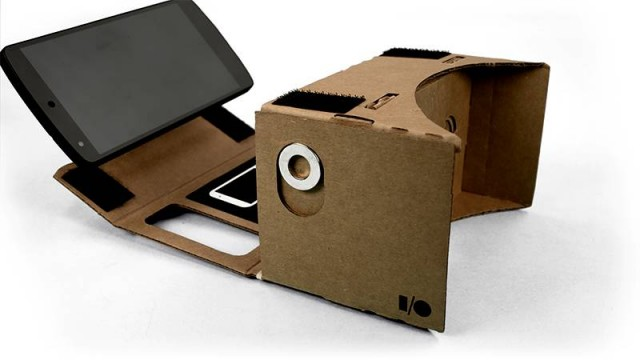
\includegraphics[width=0.7\textwidth]{res/img/cardboard1.jpg}
  \caption{Google Cardboard avec un téléphone}
\end{figure}

Juin 2014, Google dévoile Cardboard lors de sa conférence annuelle. Cet appareil en carton et plastique (lentilles) permet, à l'aide d'un smartphone que l'on insère dedans, de plonger l'utilisateur dans un environnement 3D virtuel. L'outil se présente sous la forme d'une boîte avec deux lentilles grossissantes placées entre les yeux et le téléphone disposé horizontalement. Un \og{}bouton\fg{} magnétique (aimant) offre une interaction très simpliste à l'utilisateur, disposé sur le côté gauche de l'appareil.

\subsection{Possibiltés}

\noindent Les Cardboards nous offrent principalement 4 types de projets potentiels :

\begin{itemize}
  \item Utiliser Google Maps (et donc Google StreetView) pour plonger l'utilisateur dans une planète Terre virtuelle (construite à base de photos)
  \item Créer un environnement 3D virtuel avec OpenGL ou Unity
  \item Afficher l'environnement de l'utilisateur grâce la caméra dorsale du téléphone
  \item Afficher des photos sphères (photos prises à 360° avec la caméra)
\end{itemize}
Nous avons choisi de nous orienter vers \textbf{la création d'un environnement 3D virtuel avec Unity}.

\subsection{Concept de notre projet}

\textbf{Il s'agira d'un jeu.} L'utilisateur, au départ du jeu, sera plongé dans un \textbf{labyrinthe 3D}. Le but du jeu sera simple : \textbf{sortir du labyrinthe}. Le bouton (aimant) permettra alternativement de placer le joueur en déplacement ou à l'arrêt, le choix de la direction de déplacement se faisant \og{}en réel\fg{} (le joueur devra se tourner sur lui-même pour aller à gauche ou à droite dans le jeu, cela étant possible grâce au giroscope du téléphone).

\section{Public-cible}

Ce projet s'adresse à tout type d'utilisateur disposant d'un smartphone assez récent pour être utilisé avec Google Cardboard. Il n'y pas pas de contre-indication particulière à l'usage des Cardboard. Toute personne
voulant tester la réalité virtuelle est susceptible de jouer, quelque soit son âge.

\section{Objectif}

\subsection{Objectif principal}

Notre projet consiste à créer un labyrinthe 3D dans lequel l'utilisateur serait placé, le but pour lui étant d'en sortir. Les déplacements possibles seront \og{}avancer\fg{}, \og{}tourner à droite\fg{} ou \og{}à gauche\fg{}. L'utilisateur aura également la possibilité de s'arrêter/d'avancer en utilisant l'aimant des Cardboards. Pour tourner, il suffira à l'utilisateur de réellement tourner sur lui même. Ce mouvement sera détecté grâce au gyroscope du téléphone utilisé et nous permettra de changer la direction du joueur dans le labyrinthe.

\subsection{Objectifs complémentaires}\label{sub:objectifs_complementaires}

Suivant le temps qu'il nous faudra pour prendre en main Unity (l'outil utilisé pour créer un environnement 3D), d'autres fonctionnalités pourront être envisagées telles que :
\begin{itemize}
  \item Rajouter une ambiance sonore
  \item Génération aléatoire du labyrinthe ou création de plusieurs labyrinthes, et non un seul
  \item Création d'un \textit{Pacman-like} (avec d'autres joueurs contrôlés par le téléphone -- intelligence artificielle -- poursuivants le joueur)
  \item Durée de jeu limite dans laquelle le joueur doit trouver la sortie
  \item Possibilité de jouer à plusieurs (avec plusieurs Cardboards)
  \item Possibilité d'obtenir des bonus en ramassant des objets
  \item Possibilité de plonger l'utilisateur dans le noir pendant un court instant
\end{itemize}

\subsection{Résumé}
Ce projet fait donc appel à trois types d'intéractions : \textbf{visuelles, sonores et gestuelles}. L'objectif pour nous est d'offrir une expérience immersive à l'utilisateur. Puisqu'il s'agit d'un jeu non éducatif, aucun connaissance particulière n'est apportée au joueur, seuls ses sens sont mis à l'épreuve ! De la peur et du stress pourront éventuellement naître, notamment si nous parvenons à insérer d'autres joueurs ou mettre un temps limite.

\begin{figure}[h!]
  \centering
  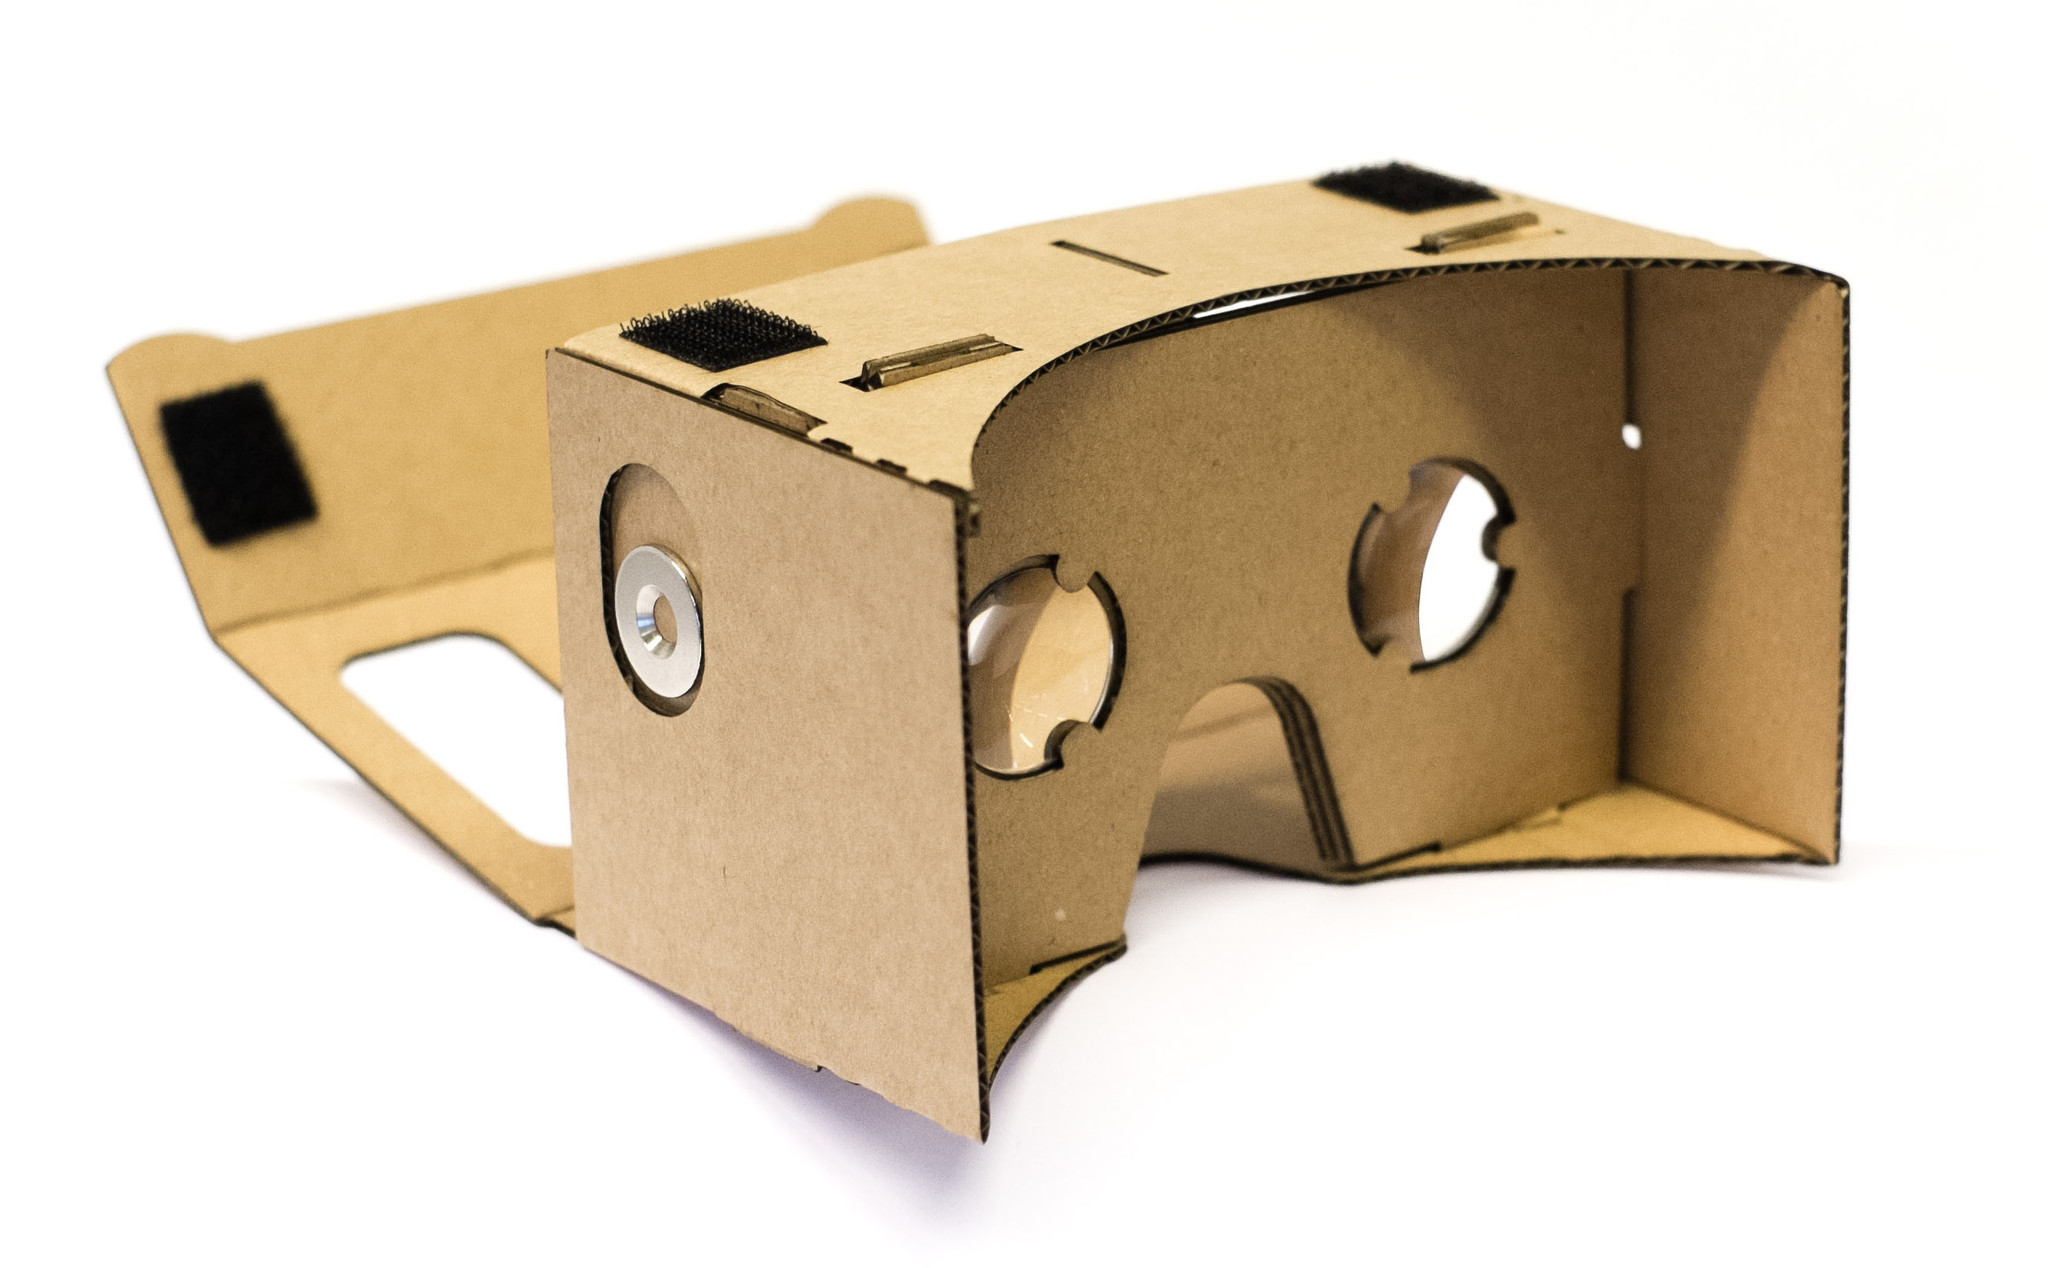
\includegraphics[width=0.4\textwidth]{res/img/cardboard2.jpg}
  \caption{Google Cardboard sans téléphone}
\end{figure}
\chapter{Cahier des charges}

\section{Budget}

Ce projet s'inscrit dans le cadre de l'UV S28, il n'y a donc pas de budget. Néanmoins, une \textbf{lourde charge de travail} est à prévoir, dûe à la découverte de Unity.

\section{Ressources médias}

Notre jeu n'utilise pas de ressource particulière de type image ou vidéo. Il s'agit uniquement d'un environnement 3D virtuel, composé de formes géométriques (les murs du labyrinthe) générées grâce au code informatique.

\medskip

En revanche, il utilisera cependant une musique de fond, \og stressante\fg{}. Cela a pour but d'\textbf{accroître l'immersion et d'accentuer l'ambiance oppressante d'un labyrinthe.}. De plus, des sons plutôt effrayants permettent de jouer sur les émotions.

\medskip

Enfin, quelques textes sont affichés à différents moments du jeu à l'utilisateur (voir chapitre \ref{scenario} du rapport ci-contre).

\medskip

D'autres éléments textuels sont susceptibles d'être ajoutés, en fonction du développement d'autres fonctionnalités (cela dépendra du temps que nous avons, cf \ref{sub:objectifs_complementaires}).

\bigskip

Ce jeu est \textbf{dynamique} : l'utilisateur est dans un environnement sur lequel il ne peut agir mais dans lequel il peut se déplacer de façon naturelle (ce n'est pas une succession d'images, ni une vidéo). Les mouvements réels du joueurs sont retransmis de manière presque naturelle dans le jeu. \textbf{La vue est à la première personne} : le joueur ne peut se voir.

\section{Structure et navigation}

Le jeu contiendra un seul type de contenu : le jeu. Il n'y a pas de menu puisqu'aucun réglage n'est proposé à l'utilisateur (pas de paramètre de jeu).

\subsection{Le jeu}
Dès le lancement de l'application sur son téléphone, le jeu démarre. Un texte apparaît : \og{}Trouvez la sortie\fg{}.

\medskip

Si le joueur désire quitter le jeu, il doit utiliser le bouton \og Retour\fg{} de son téléphone. L'écran d'accueil du téléphone apparaît alors.

\medskip

Il n'y a pas d'autre forme de navigation dans le jeu : le joueur se déplace uniquement dans un environnement virtuel 3D, comme dans un jeu vidéo, en essayant de trouver la sortie du labyrinthe dans lequel il se trouve.

\section{Formes et degrés d'interactivité}

L'interactivé réside dans l'immersion du joueur dans son environmment virtuel qu'est le labyrinthe. Il ne peut pas interagir avec en le modifiant par exemple, seulement s'y déplacer. Du vent fait mouvoir des objets (un arbre par exemple) dans le jeu, de manière à le rendre plus vivant.

\section{Choix techniques}

Notre jeu est développé pour la plateforme \textbf{Android}. Nous n'avons pas utilisé OpenGL puisque cette technologie nous était inconnue et bien trop longue à appréhender. C'est la raison pour laquelle nous nous sommes tournés vers \textbf{Unity}, qui est un moteur graphique beaucoup plus rapide à prendre en main (notamment grâce à de nombreux outils graphiques).

\medskip

Nous utilisons donc les outils fournis par Unity pour générer notre environnement 3D. Le jeu est ainsi développé dans le logiciel Unity.

\begin{figure}[h!]
  \centering
  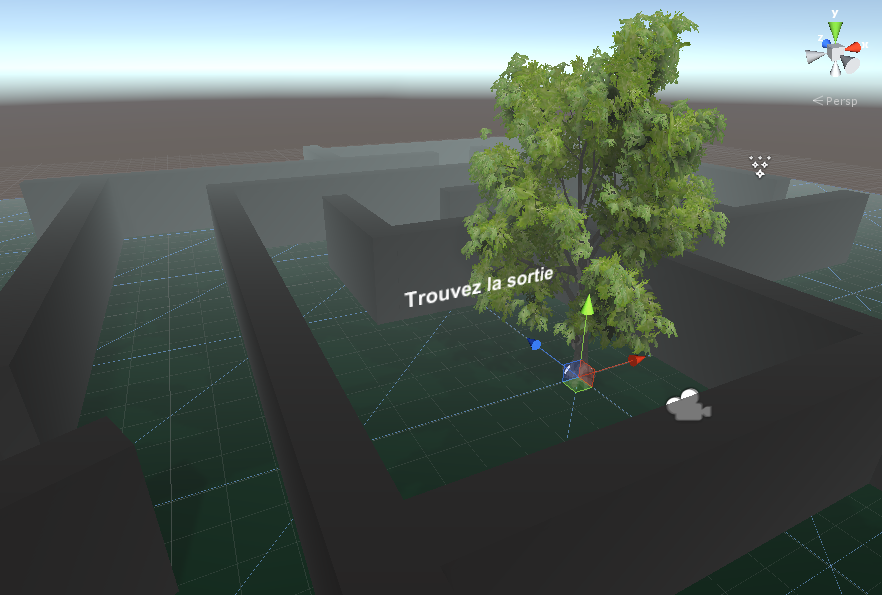
\includegraphics[width=1.0\textwidth]{res/img/unity.png}
  \caption{Création du labyrinthe sous Unity}
\end{figure}
\part{Scénario \& Storyboard}
\chapter{Scénario}\label{scenario}

\section{Textes}

Le jeu ne contient que deux phrases qui seront affichées à l'écran :
\begin{itemize}
  \item \textit{Trouvez la sortie} : affiché au tout début du jeu.
  \item \textit{Bravo ! Vous avez trouvé la sortie !} : affiché en fin de jeu, lorsque l'utilisateur parvient à trouver la sortie.
\end{itemize}

\begin{figure}[h!]
  \centering
  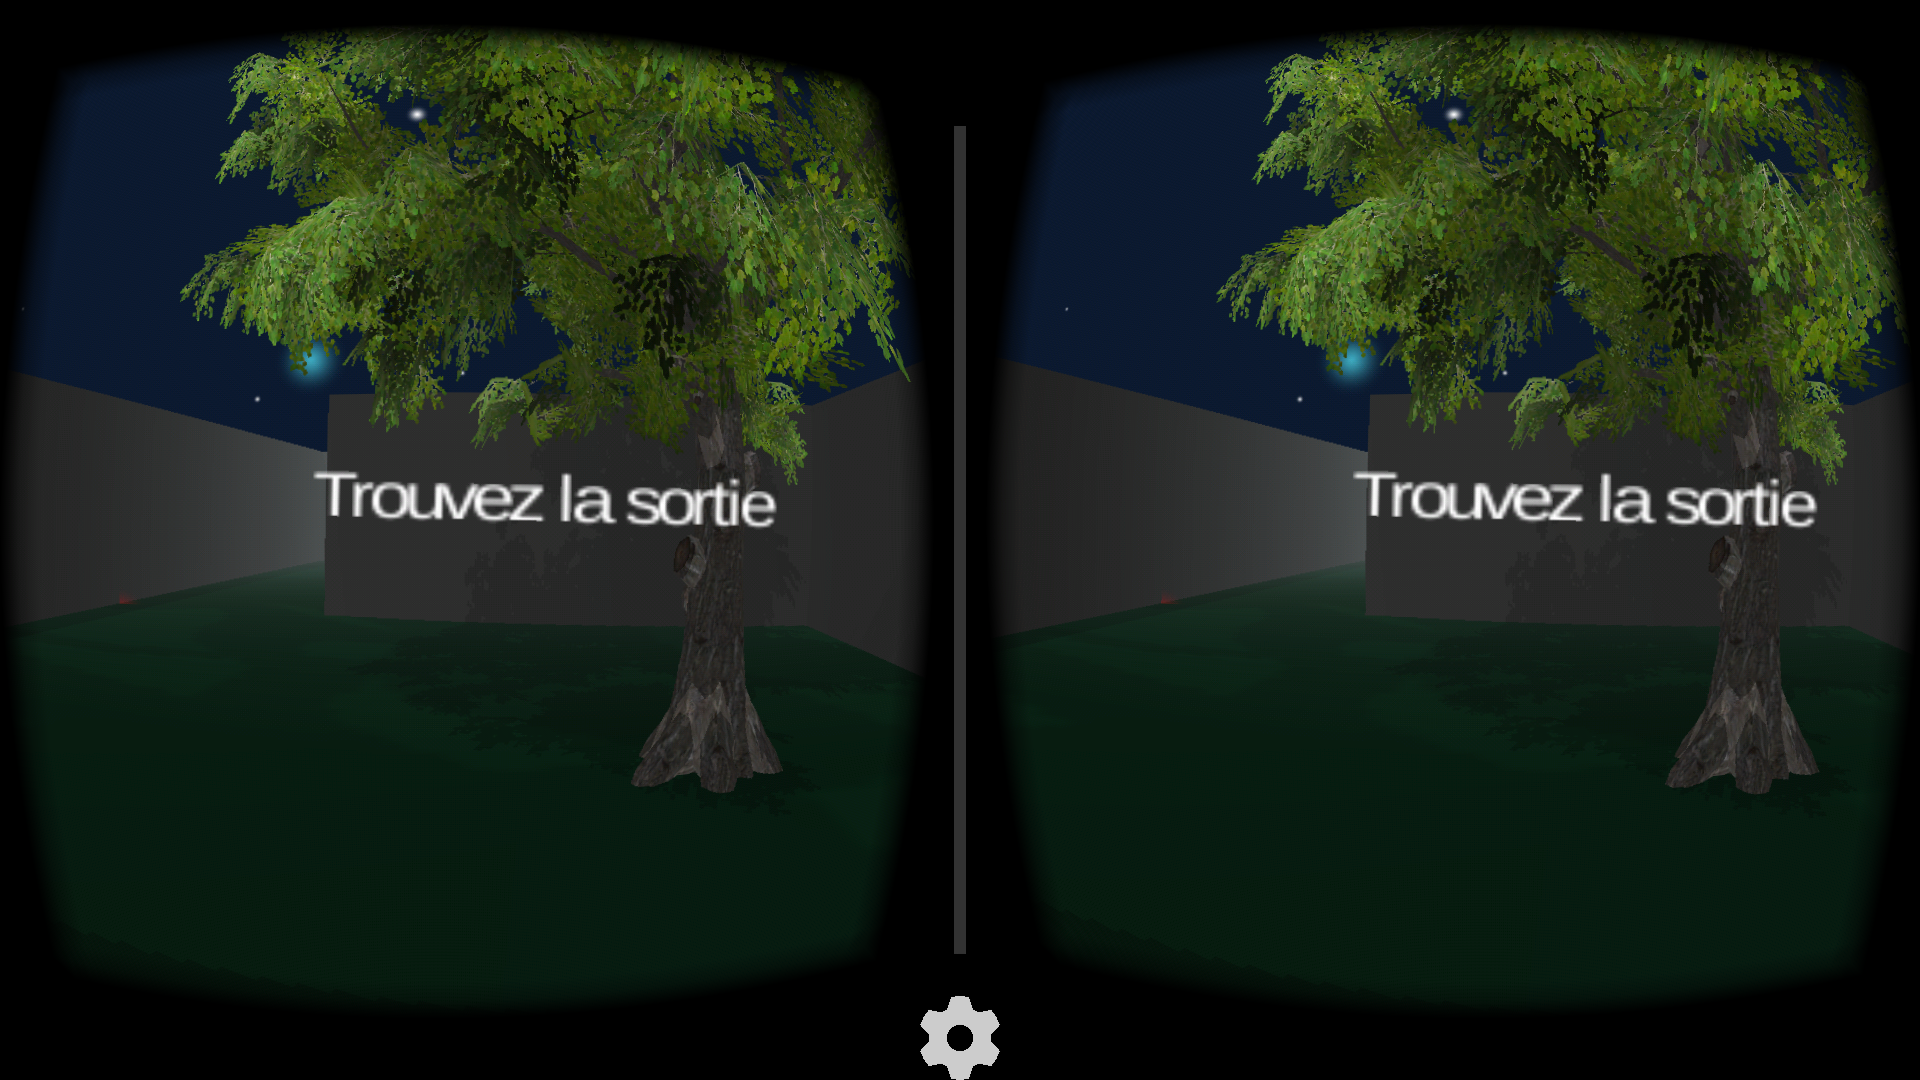
\includegraphics[width=1.0\textwidth]{res/img/trouvez-la-sortie.png}
  \caption{Démarrage du jeu}
\end{figure}

\section{Mise en scène}
Au lancement de l'application Android, le joueur est directement placé au c\oe{}ur du labyrinthe, près d'un grand arbre et son seul but est d'en sortir. Pour cela, il s'oriente vers la gauche et la droite pour tourner, tandis que son personnage fictif est à l'arrêt. La musique de fond commence immédiatement. Une action sur le bouton des Cardboard (l'aimant) permet de commencer à avancer : le joueur se déplace alors vers l'avant. Il doit donc maintenant s'orienter et parvenir à sortir du labyrinthe. Son seul répère visuel dans l'immensité du lbayrinthe est le grand arbre du début, que l'on peut apercevoir de partout.

\medskip

Des particules lumineuses volantes ainsi que du vent (qui fait mouvoir des éléments du décor, comme un arbre ou un buisson) viennent dynamiser l'environnement.

\begin{figure}[h!]
  \centering
  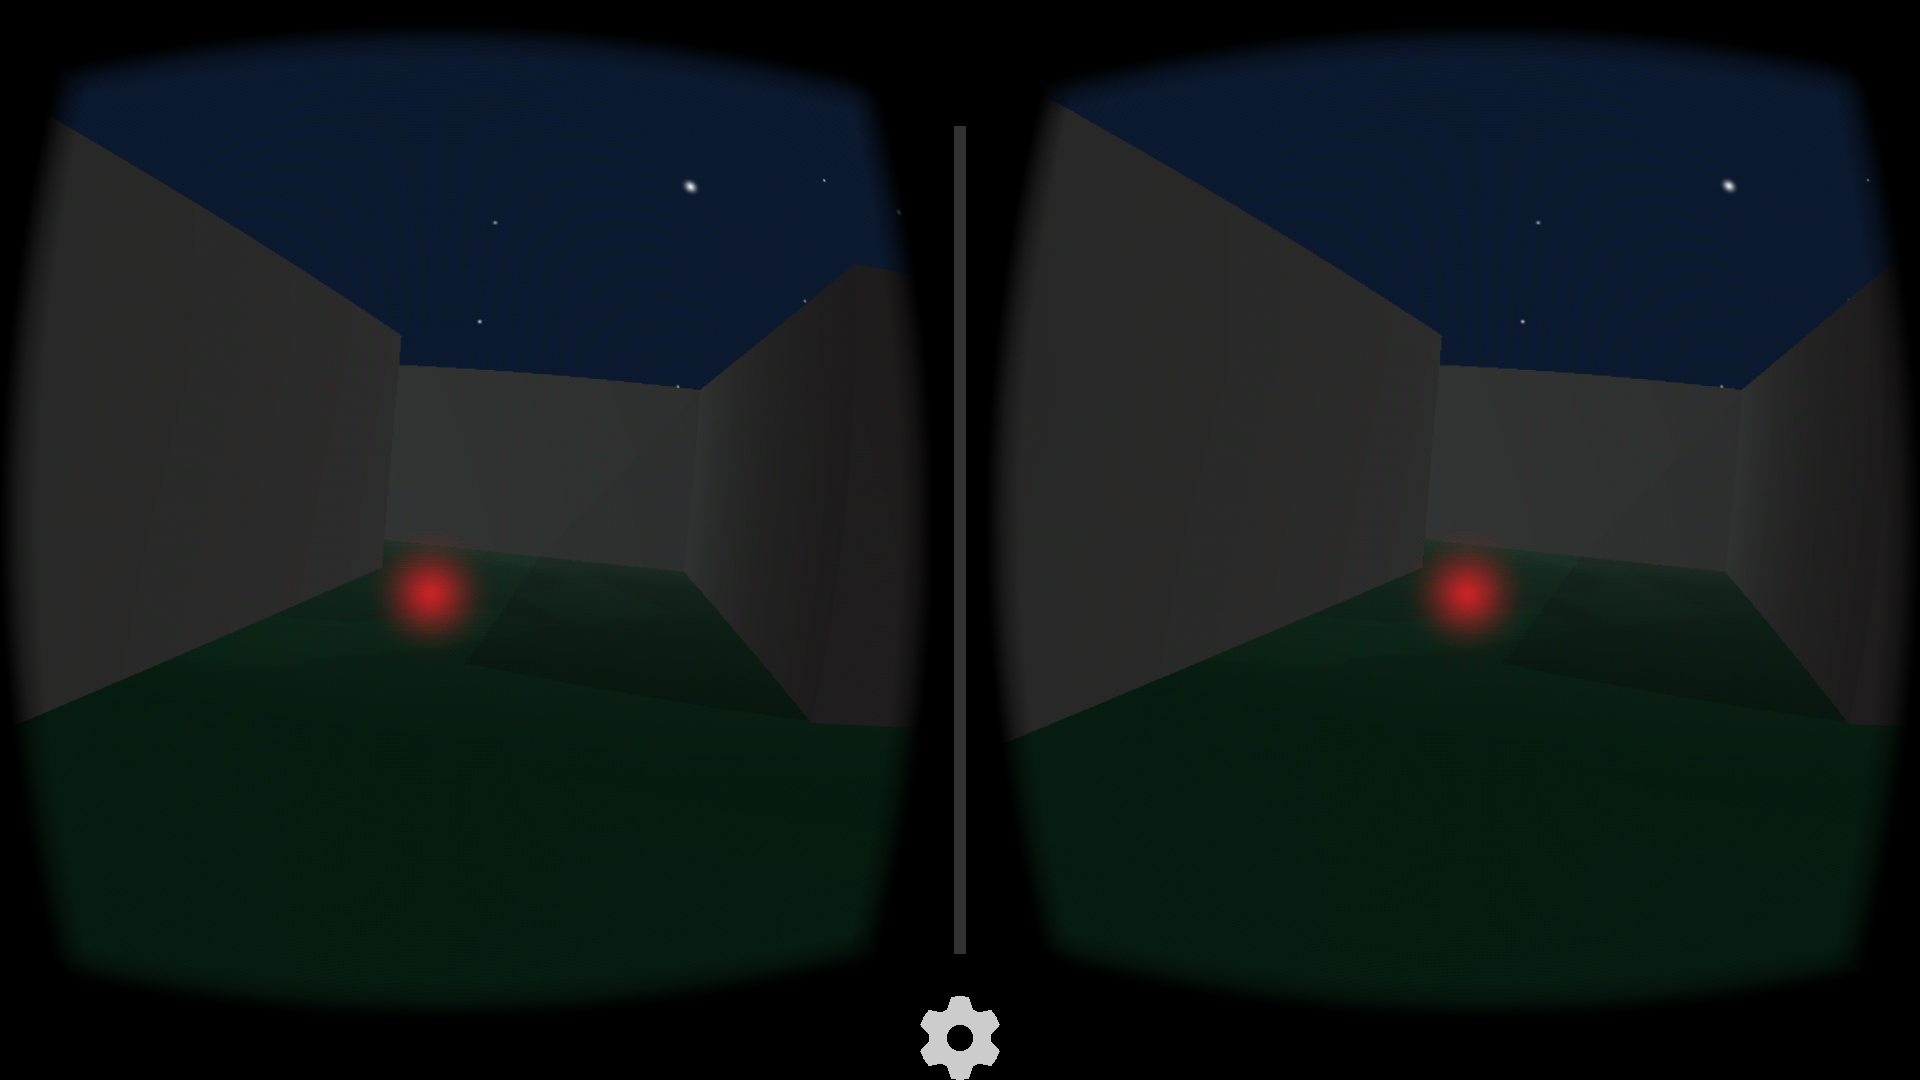
\includegraphics[width=1.0\textwidth]{res/img/couloir.png}
  \caption{Un couloir du jeu, avec des particules lumineuses volantes}
\end{figure}

\chapter{Storyboard}

\section{Charte graphique}

\subsection{Couleurs}

Le jeu est composé de couleurs sombres afin de renforcer l'ambiance oppressante du jeu. Le ciel est noir, c'est la nuit, il y a une sorte de brume. On ne distingue pas les objets au loin.

\section{Style graphique}

Il s'agit d'un jeu en 3 dimensions à la vue \og première personne\fg{}. Il n'y a pas d'animation particulière hormis des particules en suspension dans l'environnement du joueur et du vent qui souffre dans les éléments du décors (arbre, buisson).

\section{Interface graphique}

Il y a deux types d'interaction :
\begin{itemize}
  \item S'orienter (à gauche ou à droite) ; le joueur peut également regarder où bon lui semble
  \item Arrêter le mouvement : par défaut l'avatar du joueur avance en continu, il est néanmoins possible de stopper ce mouvement puis de le reprendre, cela grâce à l'aimant positionné sur le côté des Cardboard.
\end{itemize}

\medskip

\noindent L'interface graphique ne comprend pas d'HUD\footnote{\textit{Heads-Up Display : affichage tête haute, soit des informations visuelles affichées au niveau du regard}}.
\part{Conclusion}
\chapter{Conclusion générale}

\section{OpenGL ou Unity}

La plus grosse problématique du projet aura été le choix entre Unity et OpenGL. Nous étions initalement partis sur du développement en OpenGL mais heureusement, en début d'année 2015, Unity a rendu son moteur totalement gratuit, nous permettant ainsi de pouvoir l'utiliser. Nous nous en sommes rendus compte peu de temps après le début du projet et avons ainsi changé de technologie. Nous avons tout de même eu le temps d'essayer OpenGL et il s'était avéré que le développement aurait été bien trop dur et presque impossible. Effectivement, nous ne connaissions pas cette technologie et la contrainte de temps (un semestre) ne nous aurait pas permis de l'appréhender.

\section{Problèmes}

Un autre problème aura été l'utilisation du SDK de Google. Au départ nous ne savions pas comment faire déplacer le joueur, nous étions donc partis sur l'utilisation d'une \textit{library} tierce, Dive. Or il s'est avéré que cette \textit{library} souffrait d'un bug au niveau du gyroscope. Nous avons finalalement réussi à utiliser uniquement le SDK de Google et faire avancer notre joueur.

\section{Jeu final et objectifs}

Au final, un seul de nos objectifs complémentaires a été atteint : rajouter une ambiance sonore (une musique de fond). Nous sommes néanmoins très satisfaits du résultat visuel et du jeu de manière générale. Avoir plus de temps nous aurait probablement permis d'atteindre d'autres objectifs.

\end{document}
